% --------------------------------------------------------------
% This is all preamble
% --------------------------------------------------------------
 
\documentclass[10pt]{article}


% Basic Packages for Encoding (Input AND Output) and Langauge Support
\usepackage[utf8]{inputenc}
\usepackage[T1]{fontenc}
\usepackage[french]{babel}

% Change Layout with a User-Friendly Interface
\usepackage[margin=1in]{geometry} 

% Include Pictures with a User-Friendly Interface
\usepackage{graphicx}
\graphicspath{ {./images/statistics_and_probability/} }
\usepackage{float}

% Extended Math Support from the Famous 'American Mathematical Society'
\usepackage{amsmath,amsthm,amssymb}

% Section title formatting
\usepackage{titlesec}

\titleformat{\section}
            {\normalfont\scshape}{\thesection}{1em}{}

\newcommand{\N}{\mathbb{N}}
\newcommand{\Z}{\mathbb{Z}}

%Numbered Questions 
\newcounter{question}
\newenvironment{question}
               {\refstepcounter{question}\par\medskip\noindent\textbf{Q~\thequestion.}\par \noindent \rmfamily}
               {\medskip}
 
\begin{document}
 
% --------------------------------------------------------------
%                        Actual content
% --------------------------------------------------------------

\title{Exercices de révision: Statistiques et probabilité}
\author{Annie B. \thanks{Les questions sont tirées des examens de l’IB de 2018, 2012, 2011, 2010, 2007}}
\date{\today}
\maketitle

\section*{\textbf{Calculatrice Graphique Non Permise}}
%x01
\begin{question}
  \hspace*{\fill} [Note maximale: 6]\par
  \noindent Un ensemble de données comprend n valeurs.\par
  \noindent La somme des valeurs est de 800 et la moyenne est de 20\par
  \medskip
  
  (a) Trouvez n \hspace*{\fill} [2]\par
  \medskip

  \noindent L’écart type de cet ensemble de données est de 3.\par
  \noindent Chaque valeur de l’ensemble est multipliée par 10.\par
  \medskip  

  (b)\par
     \hspace{1em} (i)  Écrivez la valeur de la nouvelle moyenne. \hspace*{\fill} [2]\par
     \hspace{1em} (ii) Trouvez la valeur de la nouvelle variance.\hspace*{\fill} [2] 
\end{question}

%x02
\begin{question}
  \hspace*{\fill} [Note maximale: 14]\par
  \noindent Pablo se rend au travail en voiture.\par
  \noindent La probabilité qu’il quitte la maison avant 07 h 00 est de $\frac{3}{4}$.\par
  \noindent S'il quitte la maison avant 07 h 00, la probabilité qu’il soit en retard au travail est de $\frac{1}{8}$.\par 
  \noindent S'il quitte la maison à 07 h 00 ou après, la probabilité qu’il soit en retard au travail est de $\frac{5}{8}$.\par
  \medskip
  (a) Recopiez et complétez le diagramme en arbre suivant.\hspace*{\fill} [3]\par

  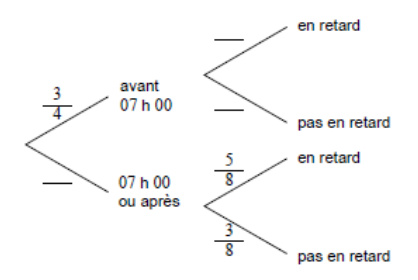
\includegraphics[scale=0.5]{q1_diagram}  

  (b) Trouvez la probabilité que Pablo quitte la maison avant 07 h 00 et qu'il soit en retard.\hspace*{\fill} [2]\par

  (c) Trouvez la probabilité que Pablo soit en retard au travail.\hspace*{\fill} [3]\par

  (d) Sachant que Pablo est en retard au travail,\par
  \hspace{1em}trouvez la probabilité qu’il ait quitté la maison avant 07 h 00.\hspace*{\fill} [3]\par

  (e) Au cours de la semaine prochaine, Pablo se rendra en voiture au travail deux jours.\par
  \hspace{1em}Trouvez la probabilité qu’il soit au moins une fois en retard.\hspace*{\fill} [3]
  
\end{question}

%x03
\begin{question}
  \hspace*{\fill} [Note maximale: 5]\par
  \noindent La courbe des effectifs cumulés ci-dessous représente les notes de 100 étudiants.\par

  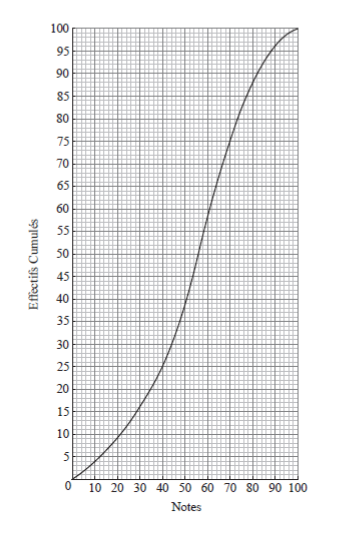
\includegraphics[scale=0.7]{courbe_de_notes}  

  (a) Trouvez la note médianne.\hspace*{\fill} [2]\par
  (b) Trouvez l'intervalle interquartile.\hspace*{\fill} [3]\par
  
\end{question}

%x04
\begin{question}
  \hspace*{\fill} [Note maximale: 8]\par
  \medskip
  \noindent La variable aléatoire X suit la distribution de probabilité suivante, avec P(X >1) = 0,5.\par

  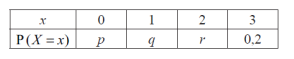
\includegraphics[scale=0.7]{px_table}  

  (a) Trouvez la valeur de r.\hspace*{\fill} [2]\par
  (b) Étant donné que E(X ) =1,4 , trouvez la valeur de p et celle de q. \hspace*{\fill} [6]\par
  
\end{question}
\newpage

%x05
\begin{question}
  \hspace*{\fill} [Note maximale: 14]\par
  \medskip
  \noindent Un sac A contient trois boules blanches et quatre boules rouges.\par
  \noindent Deux boules sont choisies au hazard et sans remise.\par
  \medskip
  (a)\par
  \hspace{1em} (i) Copiez et complétez le diagramme en arbre suivant. (N’écrivez rien sur cette page.)\par
  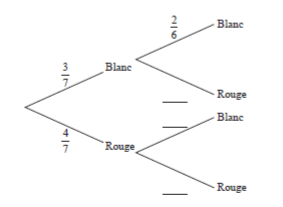
\includegraphics[scale=0.7]{arbre_rb}\par
  \hspace{1em} (ii) Trouvez la probabilité que deux boules blanches soient choisies.\hspace*{\fill} [5]\par
  \medskip  
  \noindent Un sac B contient quatre boules blanches et trois boules rouges. Quand deux boules sont choisies au hasard et sans remise dans le sac B, la probabilité qu’elles soient toutes les deux blanches est $\frac{2}{7}$\par
  \medskip
  \noindent Un dé standard est lancé. Si l’on obtient 1 ou 2, deux boules sont choisies au hasard et sans remise dans le sac A, sinon elles sont choisies dans le sac B.\par
  \medskip
  (b) Trouvez la probabilité que les deux boules soient blanches.\hspace*{\fill} [5]\par
  \medskip
  (c) Étant donné que les deux boules sont blanches,\par
  \hspace{2em} trouvez la probabilité qu’elles aient été choisies dans le sac A.\hspace*{\fill} [4]\par
  
  
\end{question}

\newpage

%x06
\begin{question}
  \hspace*{\fill} [Note maximale: 5]\par
  \medskip

  \noindent Une scientifique étudie 100 poissons femelles et 100 poissons mâles. Elle mesure 
  leur longueur (arrondie au centimètre le plus proche). Les résultats sont donnés dans
  les diagrammes à boîtes et moustache suivants.\par
  \medskip

  \noindent Poissons femelles\par
  \medskip

  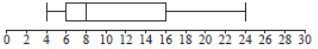
\includegraphics[scale=0.7]{poissons_femelles}\par  
  \medskip

  \noindent Poissons mâles\par
  \medskip

  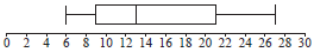
\includegraphics[scale=0.7]{poissons_males}\par  
  \medskip

  (a) Trouvez l’étendue des longueurs de tous les 200 poissons.\hspace*{\fill} [3]\par
  \medskip

  \noindent Quatre courbes de fréquence cumulée sont représentées ci-dessous.\par
  \medskip

  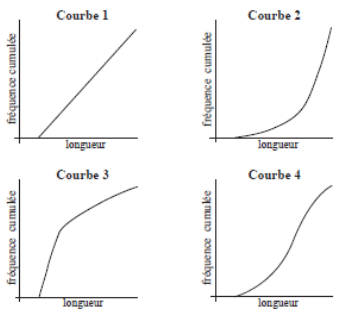
\includegraphics[scale=0.7]{courbe_1_a_4}\par  
  \medskip
  (b) Quelle courbe représente le mieux les longueurs des poissons femelles ?\hspace*{\fill} [2]\par  
\end{question}

\newpage

%x07
\begin{question}
  \hspace*{\fill} [Note maximale: 7]\par
  \medskip

  \noindent Le diagramme de Venn ci-dessous représente les événements A et B où $P(A) = 0,3$ ,\par
  
  \noindent $P(A \cup B) = 0,6 $ et $P(A \cap B) = 0,1$. Les valeurs m , n , p et q sont des probabilités. \par

  \medskip

  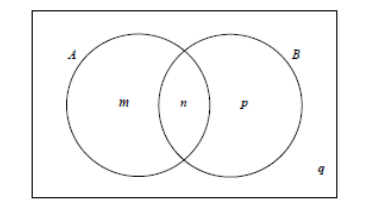
\includegraphics[scale=0.7]{venn_a_b}\par  
  \medskip
  

  (a)\par
  \hspace{2em}(i)  Donnez la valeur de n .\par
  \hspace{2em}(ii) Trouvez la valeur de m , de p et de q .\hspace*{\fill} [4]\par
  
  \medskip

  
  (b) Trouvez $P(B)$.\hspace*{\fill} [2]\par
  
\end{question}

\newpage

%x08
\begin{question}
  \hspace*{\fill} [Note maximale: 14]\par
  \medskip

  \noindent José va à l’école en bus. Chaque jour, la probabilité que José rate son bus est de $\frac{1}{3}$.\par
  \noindent S’il rate son bus, la probabilité qu’il soit en retard à l’école est de $\frac{7}{8}$.\par
  \noindent S’il ne rate pas son bus, la probabilité qu’il soit en retard est de $\frac{3}{8}$.\par
  \noindent Soit E l’événement « il rate son bus » et F l’événement « il est en retard pour l’école ».\par
  \noindent Les informations ci-dessus sont représentées dans le diagramme en arbre suivant.\par
  \medskip
  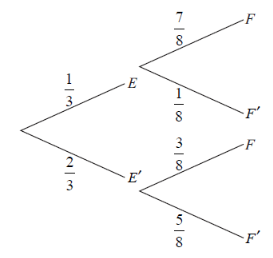
\includegraphics[scale=0.7]{arbre_e_f}\par  
  \medskip
  (a) Trouvez\par
  \hspace{2em}(i)  $P(E \cap F)$\par  
  \hspace{2em}(ii) $P(F)$\hspace*{\fill} [4]\par  
  \medskip
  (b) Trouvez la probabilité que\par
  \hspace{2em}(i)  José rate son bus et ne soit pas en retard à l’école ;\par
  \hspace{2em}(ii) José ait raté son bus, sachant qu’il est en retard à l’école.\hspace*{\fill} [5]\par
  \medskip

  \noindent Le coût pour chaque jour où José prend le bus est 3 euros.\par
  \noindent José va à l’école lundi et mardi.\par
  \medskip

  (c) Recopiez et complétez ce tableau de la distribution de probabilités.\hspace*{\fill} [3]\par
  \medskip
  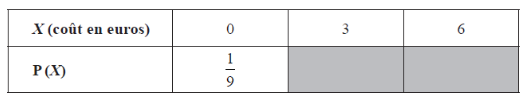
\includegraphics[scale=0.7]{tableau_cout}\par  
  \medskip
  (d) Trouvez l’espérance du coût sur les deux jours pour José.\hspace*{\fill} [2]\par
  
\end{question}
\newpage

%x09
\begin{question}
  \hspace*{\fill} [Note maximale: TBD]\par
  \medskip
  \noindent Les couleurs des yeux de 97 élèves sont données dans le tableau suivant.\par
  \medskip  
  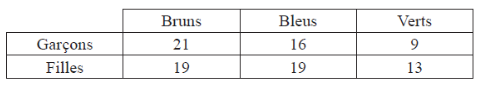
\includegraphics[scale=0.7]{tableau_yeux}\par  
  \medskip
  \noindent Un elève est choisi au hasard.\par
  (a) Donnez la probabilité que cet élève soit un garçon.\hspace*{\fill} [TBD]\par

  (b) Donnez la probabilité que cet élève ait les yeux verts, sachant qu’il s’agit d’une fille.\hspace*{\fill} [TBD]\par

  (c) Trouvez la probabilité que cet élève ait les yeux verts ou soit un garçon.\hspace*{\fill} [TBD]\par
  

\end{question}


%x10
\begin{question}
  \medskip
  \hspace*{\fill} [Note maximale: TBD]\par
  \medskip
  \noindent Les poids des enfants d’un groupe sont normalement distribués avec une moyenne de 22,5 kg
  et un écart-type de 2,2 kg.\par
  \medskip  

  (a) Donnez la probabilité qu’un enfant choisi au hasard ait un poids supérieur à 25,8 kg.\hspace*{\fill} [TBD]\par
  \medskip  

  (b) 95\% des enfants de ce groupe pèsent moins de k kilogrammes. Trouvez la valeur de k.\hspace*{\fill} [TBD]\par
  \medskip  

  (c) La figure ci-dessous représente une courbe normale.\par
  \hspace{1em}Sur cette figure, hachurez la région qui représente l’information suivante :\par
  \hspace{1em}87\% des enfants pèsent moins de 25 kg.\hspace*{\fill} [TBD]\par
  \medskip
  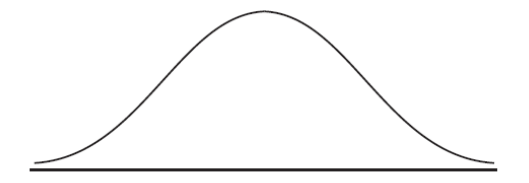
\includegraphics[scale=0.5]{courbe_normale_poids_enfants}\par  
  \medskip
\end{question}

%x11
\begin{question}
  \hspace*{\fill} [Note maximale: TBD]\par
  \medskip
  
  \noindent Un ensemble de données est: [\![ 18, 18, 19, 19, 20, 22, 22, 23, 27, 28, 28, 31, 34, 34, 36 ]\!]\par
  \noindent Le diagramme à boîtes et moustache de ces données est représenté ci-dessous.\par
  
  \medskip
  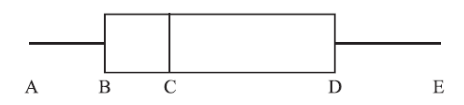
\includegraphics[scale=0.5]{boite_a_moustache_ensemble}\par  
  \medskip
  (a) Donnez les valeurs:\par
  \hspace{2em}$A =$\par
  \hspace{2em}$B =$\par
  \hspace{2em}$C =$\par
  \hspace{2em}$D =$\par
  \hspace{2em}$E =$\hspace*{\fill} [TBD]\par
  \medskip  
  (b) Trouvez l’intervalle interquartile.\hspace*{\fill} [TBD]\par
\end{question}
\newpage

\section*{\textbf{Calculatrice Graphique Permise}}

%x12
\begin{question}
  \hspace*{\fill} [Note maximale: 6]\par
  \noindent Le tableau suivant montre le poids moyen, y kg , d’enfants âgés de x ans.\par
  \medskip
  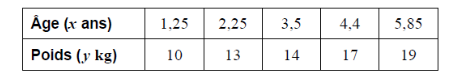
\includegraphics[scale=0.5]{tableau_age_poids}\par
  \noindent La relation entre les variables est modélisée par la droite de régression d’équation $y = ax + b$\par
  (a)\par
  \medskip
  \hspace{1em}(i)  Trouvez la valeur de a et celle de b.\par
  \medskip
  \hspace{1em}(ii) Écrivez le coefficient de corrélation.\hspace*{\fill} [4]\par
  \bigskip
  (b) Utilisez votre équation pour estimer le poids moyen d’un enfant âgé de 1,95 an.\hspace*{\fill} [2]\par
  
\end{question}

%x13
\begin{question}
  \hspace*{\fill} [Note maximale: 17]\par
  \noindent La masse M de pommes, en grammes, est normalement distribuée avec une moyenne $\mu$. Le
  tableau suivant montre les probabilités pour des valeurs de M.\par
  \medskip
  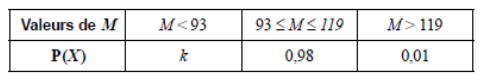
\includegraphics[scale=0.5]{tableau_de_pommes}\par
  \medskip
  (a)\par
  \medskip
  \hspace{1em}(i)  Écrivez la valeur de k.\par
  \medskip
  \hspace{1em}(ii) Montrez que $\mu = 106$.\hspace*{\fill} [4]\par
  \medskip
  (b) Trouvez $ P(M < 95)$\hspace*{\fill} [5]\par
  \medskip
  \noindent Les pommes sont emballées dans des sacs de dix.\par
  \noindent Toute pomme dont la masse est inférieure à 95 g est classée comme étant petite.\par
  \medskip
  (c) Trouvez la probabilité qu’un sac de pommes choisi au hasard contienne au plus une petite pomme.\hspace*{\fill} [3]\par
  \medskip
  (d) Une caisse contient 50 sacs de pommes. Une caisse est choisie au hasard.\par
  \medskip
  \hspace{1em}(i)  Trouvez le nombre espéré de sacs de cette caisse qui contiennent au plus une petite
pomme.\par  
  \medskip
  \hspace{1em}(ii) Trouvez la probabilité qu’au moins 48 sacs de cette caisse contiennent au plus une petite
pomme.\hspace*{\fill} [5]\par
  \bigskip

\end{question}

%x14
\begin{question}
  \hspace*{\fill} [Note maximale: 6]\par
  \medskip
  \noindent Les tailles dans un groupe d’enfants de sept ans sont normalement distribuées avec une moyenne de 117 cm et un écart-type de 5 cm. Un enfant est choisi au hasard dans ce groupe.\par
  \medskip
  (a) Trouvez la probabilité que cet enfant soit plus grand que 122,5 cm\hspace*{\fill} [3]\par
  \medskip

  (b) La probabilité que cet enfant soit plus petit que k cm est 0,65. Trouvez la valeur de k.\hspace*{\fill} [3]\par
  
\end{question}
\newpage

%x15
\begin{question}
  \hspace*{\fill} [Note maximale: 8]\par
  \medskip
  \noindent Une usine fabrique des lampes. La probabilité qu’une lampe soit défectueuse est de 0,05. Un échantillon aléatoire de 30 lampes est examiné.\par
  \medskip
  (a) Trouvez la probabilité qu’il y ait au moins une lampe défectueuse dans l’échantillon.\hspace*{\fill} [4]\par
  \medskip
  (b) Étant donné qu’il y a au moins une lampe défectueuse dans l’échantillon,\par
  \hspace{2em}trouvez la probabilité qu’il y ait au plus deux lampes défectueuses.\hspace*{\fill} [4]\par

\end{question}

%x16
\begin{question}
  \hspace*{\fill} [Note maximale: 7]\par
  \medskip
  \noindent Soit la variable aléatoire X normalement distribuée avec une moyenne de 25,\par
  \noindent comme le montre la figure ci-dessous.\par
  \medskip
  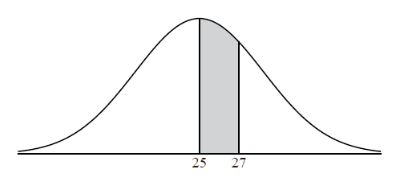
\includegraphics[scale=0.5]{normale_moyenne}\par
  \medskip
  \noindent La région grisée entre 25 et 27 représente 30\% de la distribution.\par
  \medskip
  (a) Trouvez $ P(X > 27) $\hspace*{\fill} [2]\par
  \medskip
  (b) Trouvez l’écart-type de X.\hspace*{\fill} [5]\par

\end{question}

%x17
\begin{question}
  \hspace*{\fill} [Note maximale: 12]\par
  \medskip
  \noindent Deux dés équilibrés à quatre faces, l’un rouge et l’autre vert, sont jetés. Pour chaque dé, les faces sont marquées 1, 2, 3, 4. Le score pour chaque dé est le nombre sur la face sur laquelle le dé tombe.\par
  \medskip
  (a) Listez les paires de scores qui donnent une somme de 6.\hspace*{\fill} [3]\par
  \medskip
  \noindent La distribution de probabilités pour la somme des scores des deux dés est donnée ci-dessous.\par
  \medskip
  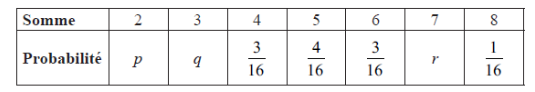
\includegraphics[scale=0.5]{tableau_sommes_des_scores}\par
  \medskip
  (b) Trouvez la valeur de p , de q et de r.\hspace*{\fill} [3]\par
  \medskip
  \noindent Fred joue à un jeu. Il lance quatre fois deux dés équilibrés à quatre faces. Il gagne un prix si la somme est 5 pour trois lancers ou plus.\par
  \medskip
  (c) Trouvez la probabilité que Fred gagne un prix.\hspace*{\fill} [6]\par
\end{question}
\newpage

%x18
\begin{question}
  \hspace*{\fill} [Note maximale: 7]\par
  \medskip
  \noindent Le tableau ci-dessous donne les notes d’examen de 120 élèves.\par
  \medskip
  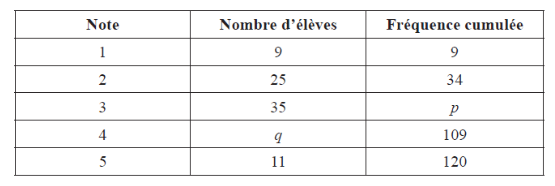
\includegraphics[scale=0.5]{histogram_etudiants_notes}\par
  (a) Trouvez la valeur de\par
  \medskip
  \hspace{2em}(i)  p.\par
  \medskip
  \hspace{2em}(ii) q.\hspace*{\fill} [4]\par
  \medskip
  (b) Trouvez la note moyenne.\hspace*{\fill} [2]\par
  \medskip
  (c) Donnez l'écart-type.\hspace*{\fill} [1]\par
\end{question}
  
%x19
\begin{question}
  \hspace*{\fill} [Note maximale: 5]\par
  \medskip
  \noindent Jan joue un jeu en jetant deux dés équilibrés à six faces. Elle gagne un lot si la somme des dés est cinq.\par
  \medskip
  (a) Jan jette les deux dés une fois. Trouvez la probabilité qu’elle gagne un lot.\hspace*{\fill} [3]\par
  \medskip
  (b) Jan jette les deux dés huit fois. Trouvez la probabilité qu’elle gagne trois lots.\hspace*{\fill} [2]\par

\end{question}

%x20
\begin{question}
  \hspace*{\fill} [Note maximale: 12]\par
  \medskip
  \noindent Il y a 50 boîtes dans une usine. Les poids, w en kg, sont divisés en 5 classes, comme le montre le tableau ci-dessous.\par
  \medskip
  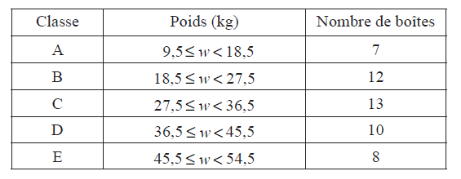
\includegraphics[scale=0.5]{tableau_poids_boite}\par
  \medskip
  (a) Montrez que le poids moyen estimé des boîtes est 32 kg.\hspace*{\fill} [3]\par
  \medskip

  (b) Dans l’usine, il y a x boîtes marquées « Fragile ». Elles sont toutes dans la\par
  \hspace{2em}classe E. Le poids moyen estimé de toutes les autres boîtes dans l’usine est 30 kg.\par
  \hspace{2em}Calculez la valeur de x.\hspace*{\fill} [4]\par
  \medskip

  (c) Une livraison de y boîtes supplémentaires, toutes ayant un poids dans la\par
  \hspace{2em}classe D, est apportée à l’usine. Le poids moyen estimé total de toutes les boîtes\par
  \hspace{2em}dans l’usine est inférieur à 33 kg . Trouvez la plus grande valeur possible de y.\hspace*{\fill} [5]\par

\end{question}
\newpage

%x21
\begin{question}
  \hspace*{\fill} [Note maximale: 16]\par
  \medskip

  \noindent Deux restaurants, Center et New, servent des sandwichs au poisson et des salades.\par
  \medskip
  \noindent Soit F l’événement « un client choisit un sandwich au poisson ».\par
  \noindent Soit S l’événement « un client choisit une salade ».\par
  \noindent Soit N l’événement « un client ne choisit ni un sandwich au poisson ni une salade ».\par
  \medskip
  \noindent Dans le restaurant Center, on a $P(F) = 0.31; P(S) = 0,62 ; P(N) = 0,14$.\par
  \medskip
  (a) Montrez que $P(F \cap S)$ = 0,07.\hspace*{\fill} [3]\par
  \medskip
  (b) Étant donné qu’un client choisit une salade, trouvez la probabilité que ce client\par
  \hspace{2em}choisisse aussi un sandwich au poisson.\hspace*{\fill} [3]\par
  \medskip
  (c) Les événements F et S sont-ils indépendants ? Justifiez votre réponse.\hspace*{\fill} [3]\par
  \medskip
  \noindent Au restaurant New, P(N) =00,.1144 . Deux fois plus de clients choisissent une salade qu’un sandwich au poisson. Choisir un sandwich au poisson est indépendant de choisir une salade.\par
  \medskip
  (d) Trouvez la probabilité de choisir un sandwich au poisson.\hspace*{\fill} [7]\par
  
\end{question}

\end{document}
